% Template for Cogsci submission with R Markdown

% Stuff changed from original Markdown PLOS Template
\documentclass[10pt, letterpaper]{article}

\usepackage{cogsci}
\usepackage{pslatex}
\usepackage{float}
\usepackage{caption}

% amsmath package, useful for mathematical formulas
\usepackage{amsmath}

% amssymb package, useful for mathematical symbols
\usepackage{amssymb}

% hyperref package, useful for hyperlinks
\usepackage{hyperref}

% graphicx package, useful for including eps and pdf graphics
% include graphics with the command \includegraphics
\usepackage{graphicx}

% Sweave(-like)
\usepackage{fancyvrb}
\DefineVerbatimEnvironment{Sinput}{Verbatim}{fontshape=sl}
\DefineVerbatimEnvironment{Soutput}{Verbatim}{}
\DefineVerbatimEnvironment{Scode}{Verbatim}{fontshape=sl}
\newenvironment{Schunk}{}{}
\DefineVerbatimEnvironment{Code}{Verbatim}{}
\DefineVerbatimEnvironment{CodeInput}{Verbatim}{fontshape=sl}
\DefineVerbatimEnvironment{CodeOutput}{Verbatim}{}
\newenvironment{CodeChunk}{}{}

% cite package, to clean up citations in the main text. Do not remove.
\usepackage{cite}

\usepackage{color}

% Use doublespacing - comment out for single spacing
%\usepackage{setspace}
%\doublespacing


% % Text layout
% \topmargin 0.0cm
% \oddsidemargin 0.5cm
% \evensidemargin 0.5cm
% \textwidth 16cm
% \textheight 21cm

\title{Communicative pressure can lead to input that supports language learning}


\author{{\large \bf Benjamin C. Morris} \\ \texttt{benmorris1@uchicago.edu} \\ Department of Psychology \\ University of Chicago \And {\large \bf Daniel Yurovsky} \\ \texttt{yurovsky@uchicago.edu} \\ Department of Psychology \\ University of Chicago}

\begin{document}

\maketitle

\begin{abstract}
The abstract should be one paragraph, indented 1/8 inch on both sides,
in 9 point font with single spacing. The heading Abstract should be 10
point, bold, centered, with one line space below it. This one-paragraph
abstract section is required only for standard spoken papers and
standard posters (i.e., those presentations that will be represented by
six page papers in the Proceedings).

\textbf{Keywords:}
Add your choice of indexing terms or keywords; kindly use a semi-colon;
between each term.
\end{abstract}

\section{Introduction}\label{introduction}

One of the most striking aspects of children's language learning is just
who quickly they master the complex system of their natural langauge
(Bloom, 2000). In just a few short years, children go from complete
ignorance to conversational fluency that is the envy of second-language
learners attempting the same feat later in life (Newport, 1990). What
accounts for this remarkable transition?

One possiblility is that children's caregivers deserve most of the
credit; that the language parents produce to their children is optimized
for teaching. Although there is some evidence that aspects of
child-directed support learning, other aspects--even in the same
subproblem, e.g.~phoneme discrimination--appear to make learning more
difficulty (Eaves Jr, Feldman, Griffiths, \& Shafto, 2016; McMurray,
Kovack-Lesh, Goodwin, \& McEchron, 2013). In general, parents rarely
explicltly correct their children, and children are resistant to the
rare explicit language correction they do get (Newport, Gleitman, \&
Gleitman, 1977). Thus while parents may occasionally offer a supervisory
signal, the bulk of the evidence suggests that parental supervision is
unlikely to explain rapid early language acqusition.

Alternatively, even the youngest infants may already come to language
acquisition with a precocious ability to learn the latent structure of
language from the statistical properties of the language in their
ambient environment (Saffran \& 2003, 2003; L. B. Smith \& Yu, 2008).
While a number of experiments clearly demonstrate the early availability
of such mechanisms, there is reason to be suspicious about just how
precocious they are early in development. For example, infants' ability
to track the co-occurrence information connecting words to their
referents appears to be highly constrained by both their developing
memory and attention systems {[}Vlach \& Johnson (2013);smith2013{]}.
Further, computational models of these processes show that the rate of
acquisition is highly sensitive to variation in environmental statistics
(Blythe, Smith, \& Smith, 2010; Vogt, 2012). Thus precocious
unsupervised statistical learning also appears to fall short of an
explanation for rapid early language learning.

In this paper we explore the consequences of a a third possibility: The
language that children hear is neither designed for pedagogy, nor is it
random: it is designed for communication (Brown, 1977). We take as the
caregiver's goal the desire to communicate with the child, not about
language itself, but instead about the world in front of them. To
succeed, the caregiver must produce the kinds of commincative signals
that the child can understand, and thus might tune the complexity of
their speech not for the sake of learning itself, but as a byproduct of
in-the-moment pressure to communicate successfully (Yurovsky, 2017).

We take as our model system a simple iterated reference game in which
two players earn points for communicating successfully with each-other
about the objects in front of them. First in a computational model, and
then in a set of experiments with adults on Mechanical Turk, we show
that pedagogically-supportive input can arise from purely selfish
motives to maximize the cost of communicating successfully while
minimizing the cost of communcation. We take these results as a proof of
concept that both the features of child-directed speech that support
learning as well as those that inhibit it may arise from a single
unifying goal: The desire to communicative efficiently.

For general information about authoring in markdown, see
\textbf{\href{http://rmarkdown.rstudio.com/authoring_basics.html}{here}.}

For standard spoken papers and standard posters, the entire contribution
(including figures, references, everything) can be no longer than six
pages. For abstract posters, the entire contribution can be no longer
than one page. For symposia, the entire contribution can be no longer
than two pages.

The text of the paper should be formatted in two columns with an overall
width of 7 inches (17.8 cm) and length of 9.25 inches (23.5 cm), with
0.25 inches between the columns. Leave two line spaces between the last
author listed and the text of the paper. The left margin should be 0.75
inches and the top margin should be 1 inch.
\textbf{The right and bottom margins will depend on whether you use
U.S. letter or A4 paper, so you must be sure to measure the width of
the printed text.} Use 10 point Times Roman with 12 point vertical
spacing, unless otherwise specified.

The title should be in 14 point, bold, and centered. The title should be
formatted with initial caps (the first letter of content words
capitalized and the rest lower case). Each author's name should appear
on a separate line, 11 point bold, and centered, with the author's email
address in parentheses. Under each author's name list the author's
affiliation and postal address in ordinary 10 point type.

Indent the first line of each paragraph by 1/8\textasciitilde{}inch
(except for the first paragraph of a new section). Do not add extra
vertical space between paragraphs.

\section{First-Level Headings}\label{first-level-headings}

First level headings should be in 12 point , initial caps, bold and
centered. Leave one line space above the heading and
1/4\textasciitilde{}line space below the heading.

\subsection{Second-Level Headings}\label{second-level-headings}

Second level headings should be 11 point , initial caps, bold, and flush
left. Leave one line space above the heading and 1/4\textasciitilde{}
line space below the heading.

\subsubsection{Third-Level Headings}\label{third-level-headings}

Third-level headings should be 10 point , initial caps, bold, and flush
left. Leave one line space above the heading, but no space after the
heading.

\section{Formalities, Footnotes, and
Floats}\label{formalities-footnotes-and-floats}

Use standard APA citation format. Citations within the text should
include the author's last name and year. If the authors' names are
included in the sentence, place only the year in parentheses, as in
({\textbf{???}}), but otherwise place the entire reference in
parentheses with the authors and year separated by a comma
({\textbf{???}}). List multiple references alphabetically and separate
them by semicolons ({\textbf{???}}, {\textbf{???}}). Use the et. al.
construction only after listing all the authors to a publication in an
earlier reference and for citations with four or more authors.

For more information on citations in R Markdown, see
\textbf{\href{http://rmarkdown.rstudio.com/authoring_bibliographies_and_citations.html\#citations}{here}.}

\subsection{Footnotes}\label{footnotes}

Indicate footnotes with a number\footnote{Sample of the first
footnote.} in the text. Place the footnotes in 9 point type at the
bottom of the page on which they appear. Precede the footnote with a
horizontal rule.\footnote{Sample of the second footnote.}

\subsection{Figures}\label{figures}

All artwork must be very dark for purposes of reproduction and should
not be hand drawn. Number figures sequentially, placing the figure
number and caption, in 10 point, after the figure with one line space
above the caption and one line space below it. If necessary, leave extra
white space at the bottom of the page to avoid splitting the figure and
figure caption. You may float figures to the top or bottom of a column,
or set wide figures across both columns.

\subsection{Two-column images}\label{two-column-images}

You can read local images using png package for example and plot it like
a regular plot using grid.raster from the grid package. With this method
you have full control of the size of your image. \textbf{Note: Image
must be in .png file format for the readPNG function to work.}

You might want to display a wide figure across both columns. To do this,
you change the \texttt{fig.env} chunk option to \texttt{figure*}. To
align the image in the center of the page, set \texttt{fig.align} option
to \texttt{center}. To format the width of your caption text, you set
the \texttt{num.cols.cap} option to \texttt{2}.

\begin{CodeChunk}
\captionsetup{width=0.8\textwidth}\begin{figure*}[h]

{\centering 
\includegraphics{figs/2-col-image-1} 

}

\caption[This image spans both columns]{This image spans both columns. And the caption text is limited to 0.8 of the width of the document.}\label{fig:2-col-image}
\end{figure*}
\end{CodeChunk}

\subsection{One-column images}\label{one-column-images}

Single column is the default option, but if you want set it explicitly,
set \texttt{fig.env} to \texttt{figure}. Notice that the
\texttt{num.cols} option for the caption width is set to \texttt{1}.

\begin{CodeChunk}
\captionsetup{width=0.8\columnwidth}\begin{figure}[H]

{\centering 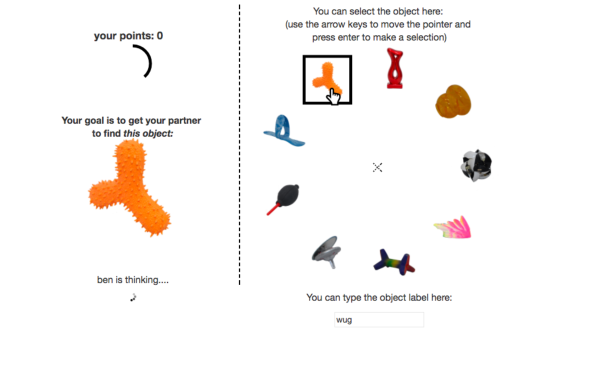
\includegraphics{figs/image-1} 

}

\caption[One column image]{One column image.}\label{fig:image}
\end{figure}
\end{CodeChunk}

\subsection{R Plots}\label{r-plots}

You can use R chunks directly to plot graphs. And you can use latex
floats in the fig.pos chunk option to have more control over the
location of your plot on the page. For more information on latex
placement specifiers see
\textbf{\href{https://en.wikibooks.org/wiki/LaTeX/Floats,_Figures_and_Captions}{here}}

\begin{CodeChunk}
\begin{figure}[H]

{\centering 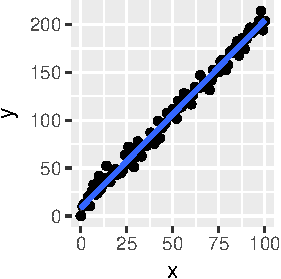
\includegraphics{figs/plot-1} 

}

\caption[R plot]{R plot}\label{fig:plot}
\end{figure}
\end{CodeChunk}

\subsection{Tables}\label{tables}

Number tables consecutively; place the table number and title (in 10
point) above the table with one line space above the caption and one
line space below it, as in Table 1. You may float tables to the top or
bottom of a column, set wide tables across both columns.

You can use the xtable function in the xtable package.

\begin{table}[H]
\centering
\begin{tabular}{rrrrr}
  \hline
 & Estimate & Std. Error & t value & Pr($>$$|$t$|$) \\ 
  \hline
(Intercept) & 0.08 & 0.09 & 0.9 & 0.38 \\ 
  x & 2.15 & 0.10 & 20.9 & 0.00 \\ 
   \hline
\end{tabular}
\caption{This table prints across one column.} 
\end{table}

\section{Acknowledgements}\label{acknowledgements}

Place acknowledgments (including funding information) in a section at
the end of the paper.

\section{References}\label{references}

\setlength{\parindent}{-0.1in} \setlength{\leftskip}{0.125in} \noindent

\hypertarget{refs}{}
\hypertarget{ref-bloom2000}{}
Bloom, P. (2000). \emph{How children learn the meanings of words}. MIT
press: Cambridge, MA.

\hypertarget{ref-blythe2010}{}
Blythe, R. A., Smith, K., \& Smith, A. D. M. (2010). Learning times for
large lexicons through cross-situational learning. \emph{Cognitive
Science}, \emph{34}, 620--642.

\hypertarget{ref-brown1977}{}
Brown, R. (1977). Introduction. In C. E. Snow \& C. A. Ferguson (Eds.),
\emph{Talking to children: Language input and interaction}. Cambridge,
MA.: MIT Press.

\hypertarget{ref-eaves-jr2016}{}
Eaves Jr, B. S., Feldman, N. H., Griffiths, T. L., \& Shafto, P. (2016).
Infant-directed speech is consistent with teaching. \emph{Psychological
Review}, \emph{123}(6), 758.

\hypertarget{ref-mcmurray2013}{}
McMurray, B., Kovack-Lesh, K. A., Goodwin, D., \& McEchron, W. (2013).
Infant directed speech and the development of speech perception:
Enhancing development or an unintended consequence? \emph{Cognition},
\emph{129}(2), 362--378.

\hypertarget{ref-newport1990}{}
Newport, E. L. (1990). Maturational Constraints on Language Learning.
\emph{Cognitive Science}, \emph{14}(1), 11--28.

\hypertarget{ref-newport1977}{}
Newport, E. L., Gleitman, H., \& Gleitman, L. R. (1977). Mother, I'd
rather do it myself: Some effects and non-effects of maternal speech
style. In C. A. Ferguson (Ed.), \emph{Talking to children language input
and interaction} (pp. 109--149). Cambridge University Press.

\hypertarget{ref-saffran2003}{}
Saffran, J. R., \& 2003. (2003). Statistical language learning:
Mechanisms and constraints. \emph{Current Directions in Psychological
Science}, \emph{12}(4), 110--114.

\hypertarget{ref-smith2008}{}
Smith, L. B., \& Yu, C. (2008). Infants rapidly learn word-referent
mappings via cross-situational statistics. \emph{Cognition}, \emph{106},
1558--1568.

\hypertarget{ref-vlach2013}{}
Vlach, H. A., \& Johnson, S. P. (2013). Memory constraints on infants’
cross-situational statistical learning. \emph{Cognition}, \emph{127}(3),
375--382.

\hypertarget{ref-vogt2012}{}
Vogt, P. (2012). Exploring the robustness of cross-situational learning
under zipfian distributions. \emph{Cognitive Science}, \emph{36}(4),
726--739.

\hypertarget{ref-yurovsky2017}{}
Yurovsky, D. (2017). A communicative approach to early word learning.
\emph{New Ideas in Psychology}, 1--7.

\end{document}
